\documentclass[12pt]{report}
\usepackage{amsmath}
\usepackage{amssymb}
\usepackage{graphicx}
\usepackage{longtable}
\usepackage{tikz}

\newcommand{\bt}[1]{\textbf{#1}}
\newcommand{\ubt}[1]{\textbf{\underline{#1}}}
\newcommand{\sps}{\\[0.2cm]}
\newcommand{\spn}[1]{\\[#1cm]}
\newcommand{\refn}[1]{(\ref{#1})}
\newcommand{\refx}[1]{\refn{eq:#1}}
\newcommand{\NI}{\noindent}
\newcommand{\dsp}{\displaystyle}
\newcommand{\sprime}{'}
\newcommand{\dprime}{''}
\newcommand{\tprime}{'''}
\newcommand{\tti}[1]{\textit{#1}}


\renewcommand*\contentsname{Table of Contents}
\renewcommand{\baselinestretch}{1.1}

\begin{document}
	%%remove the numbering from the first page 
	\clearpage
	\thispagestyle{empty}
	%%TITLE%%
	\addcontentsline{toc}{chapter}{TITLE PAGE}
	\begin{center}
		{\bf \Large FINITE DIFFERENCE METHOD FOR SOLVING ORDINARY DIFFERENTIAL EQUATIONS }
	\end{center}
	$$$$
	\begin{center}
		\textbf{\itshape BY}
	\end{center} 
	$$$$
	\begin{center}
		{\bf ALAO, Habeeb Omotola\\
			16/56EB042}
	\end{center}
	$$$$
	\begin{center}
		\textbf{A PROJECT SUBMITTED TO THE
			DEPARTMENT OF MATHEMATICS, FACULTY OF PHYSICAL SCIENCES,
			UNIVERSITY OF ILORIN, ILORIN, NIGERIA,
			$$$$
			IN PARTIAL 
			FULFILMENT OF REQUIREMENTS FOR THE AWARD OF
			BACHELOR OF SCIENCE (B.Sc.) DEGREE IN MATHEMATICS.}
	\end{center}
	$$ $$ 
	\\ \\
	\begin{center}
		{\bf JUNE, 2021}
	\end{center}
	\newpage
	\pagenumbering{roman} 
	\addcontentsline{toc}{chapter}{CERTIFICATION}
	\section*{\begin{center}\textbf{\Large CERTIFICATION}   \end{center}}
	This is to certify that this project work was carried out by \textbf{ALAO, Habeeb Omotola} with matriculation number \textbf{16/56EB042} and approved as meeting the requirement for the award of the Bachelor of Science (B. Sc.) degree of the Department of Mathematics, Faculty of Physical Sciences, University of Ilorin, Ilorin, Nigeria.
	\\
	\\
	................................... \quad \qquad\qquad\qquad\qquad\quad...................... \\
	Dr. K. A. Bello  \qquad\qquad\qquad\qquad\qquad\qquad\qquad Date\\
	Supervisor\\
	\\
	\\
	\\
	.................................... \qquad\qquad\qquad\qquad\qquad......................\\
	Prof. K. Rauf      \qquad\qquad\qquad\qquad\qquad\qquad\qquad\quad     Date\\
	Head of Department\\
	\\
	\\
	\\
	..................................... \qquad\qquad\qquad\qquad\qquad.......................\\
	Prof. T. O. Oluyo  \qquad\qquad\qquad\qquad\qquad\qquad \quad        Date\\
	External Examiner
	
	\newpage
	%%DEDICATION%%
	\section*{\begin{center}	\textbf{\Large DEDICATION}   \end{center}}
	\addcontentsline{toc}{chapter}{DEDICATION}
	This project work is dedicated to my Parents; Mr. and Mrs. Moshood Alao.
	
	\newpage
	%%ACKNOLEDGEMENT%%
	\section*{\begin{center}\textbf{\Large ACKNOWLEDGMENTS}\end{center}}
	\addcontentsline{toc}{chapter}{ACKNOWLEDGMENTS} 					
	Thanks to almighty Allah the king of the universe, the most merciful, gracious and all forgiving and also peace be upon the prophet Muhammad (S.A.W) and his companions (Ameen). I give thanks to almighty Allah for seeing me through all these years of study.\\
	
	\NI My profound gratitude goes to my supervisor. Dr K. A Bello for his support through the supervision. May almighty Allah support and be with him and his family. \\
	
	\NI I also appreciate the immeasurable effort of my lecturers in the department; Professors J. A Gbadeyan, O. T. Opoola, O. M. Bamigbola, M. O. Ibrahim, O. A. Taiwo, R. B. Adeniyi, A. S. Idowu, M. S. Dada, K. O. Babalola and Doctors E.O. Titiloye,  Olubunmi A. Fadipe-Joseph, Dr. Yidiat O. Aderinto, Dr. Catherine N. Ejieji, Dr. B. M. Yisa, Dr J. U. Abubakar, Dr. Gata N. Bakare, Dr T. O. Olotu, Dr. B. M. Ahmed, Dr Idayat F. Usamot, Dr O. A. Uwaheren, O. Odetunde and all other members of staff of the department of mathematics, who contributed greatly to my academic excellence, obtained during my period of study in the department. May God bless them all.\\
	%My appreciation also goes to the Head of department Professor K. Rauf and my level adviser; Dr. I. F. Usamot, for their useful guidelines and advices throughout my stay in the university. I equally appreciate the efforts of all my lecturers in the department; Professors J. A. Gbadeyan, T. O. Opoola, O. M. Bamigbola, M. O. Ibrahim, O. A. Taiwo, R. B. Adeniyi, A. S. Idowu, M. S. Dada, K. O. Babalola, and Drs. J. U. Abubakar, E. O. Titiloye. O. A. Fadipe Joseph, Y. O. Aderinto, C. N. Ejieji, B. M. Yisa, G. N. Bakare, B. M. Ahmed, T. I. Oyekunle, O. Odetunde and all other staff of the department.\\
	
	\NI I am highly indebted to my loving and caring family especially my parents, Mr. and Mrs. Moshood Alao for their prayers, and unparallel support. To all my siblings; Mubarak, Abdul Rasaq, Mustapha, Habeebat, Azeezat, and Barakat, I say thank you for all your tolerance and patience with me all over the years.\\
	
	\NI To my friends in the department; to mention few, Joseph Adeola, Sodiq, and Uthman, big shout
	out to you all and thank you for your assistance and inputs during my course work and in this
	project. May our paths always be smooth and favour-filled.
	God bless you all.\\
	
	
	\newpage
	%%ABSTRACT%%
	\section*{\begin{center}\textbf{\Large ABSTRACT}\end{center}}
	\addcontentsline{toc}{chapter}{ABSTRACT}
	In this project, Finite Difference Method (FDM) is applied to solve second order Ordinary Differential Equations (ODEs). The method assumed an approximate solution using the Taylor’s series as basis function which are then substituted into the problem considered. Four (4) examples were considered to illustrate the accuracy of the FDM. Also, errors of the problem is presented in tabular form.
	
	%%TABLE OF CONTENTS%%
	\addcontentsline{toc}{chapter}{TABLE OF CONTENTS}
	\tableofcontents
	\newpage
	
	\pagenumbering{arabic}
	%%%%%%%%%%%%%%%%%%%%%%%%%CHAPTER ONE%%%%%%%%%%%%%%%%%%%%%%%%%%%%
	\chapter{GENERAL INTRODUCTION}
	
	\section{Background to the Study}
	For the past years, the problem of the classical boundary layer over a surface has been studied in two different types. First is a boundary layer flow past a stationary surface, while the other type is
	the problem of a boundary layer flow over a solid surface continuously moving in a fluid at rest such as hot rolling, metal forming and continuous casting.\sps
	Finite difference methods for partial differential equations (PDEs) employ a range of concepts and tools that can be introduced and illustrated in the context of simple ordinary differential equation
	(ODE) examples. By first working with ODEs, mathematical problems to be solved is tailored in such a way to be in simple form as possible thereby allowing full focus on understanding the concepts and tools that will be reused and further extended when addressing finite difference methods for time-dependent PDEs. The forthcoming treatment of ODEs is therefore solely dominated by reasoning and methods that directly carry over to numerical methods for PDEs.\sps
	Several models could be solved in ODE using finite elements. Notable among them are an ODE for a decaying phenomenon, which will be relevant for PDEs of diffusive nature, and an ODE for oscillating phenomena, which will be relevant for PDEs of wave nature. These problems are linear with known analytical solutions such that the quality of various numerical methods and behavior
	could be easily analysed.
	
	\section{Definition of Relevant Terms}
	
	\subsection{Differential Equations}
	Differential equation is otherwise known as mathematical equation. In this case, there exists an unknown function of one variable or more which relates the value of the function to itself and its derivatives of various order.
	\begin{equation}
		a_x(x)\frac{d^nx}{dx^n} + a_{n-1}(x)\frac{d^{n-1}y}{dx^{n-1}} + \cdots + a_1(x)\frac{dy}{dx} + a_0(x)y = g(x) \label{eq:1_1}
	\end{equation}
	Example of a differential equation is $y\dprime -2y\sprime + y = 0$\sps
	Differential equation can be classified by type, order, and linearity. The classification by type are Ordinary Differential Equation (ODE) and Partial Differential Equation (PDE) while differential equation by order. Classification by type and linearity is in the nth form; and linear/non-linear forms respectively.
	\newpage
	
	\subsection{Ordinary Differential Equation}
	Any equation with only one dependent variable is known as an ODE. An example of such is given in the equation below.
	\begin{equation}
		\frac{dy}{dx} = 5x + 25 \label{eq:1_2}
	\end{equation}
	
	\subsection{Partial Differential Equation}
	Any equation with more than one independent variable is call a PDE. An example of such is given in the equation below.
	\begin{equation}
		\frac{\partial z}{\partial x} + \frac{\partial z}{\partial y} = x^2 \label{eq:1_3}
	\end{equation}
	
	\subsection{Normal Form Differential Equation}
	Normal form differential equation is the order of differential equation with the highest derivative. $nth$-order ODE is given below as
	\begin{equation*}
		F(x,y,y\sprime,\ldots,y^{(n)}) = 0
	\end{equation*}
	The normal form is therefore
	\begin{equation}
			\frac{d^ny}{dx^n}=f(x,y,y\sprime,\ldots,y^{(n-1)}) \label{eq:1_4}
	\end{equation}
	
	\subsection{Linear or Non-Linear Differential Equation}
	A $nth$-order ODE is said to be linear if it can be written in the form below
	\begin{equation}
		a_x(x)\frac{d^nx}{dx^n} + a_{n-1}(x)\frac{d^{n-1}y}{dx^{n-1}} + \cdots + a_1(x)\frac{dy}{dx} + a_0(x)y = g(x) \label{eq:1_5}
	\end{equation}
	A linear differential equation is any differential equation that can be written in the following form.
	\begin{equation*}
		a_n(t)y^{(n)}(t) + a_{n-1}(t)y^{(n-1)}(t) + \cdots + a_1(t)y\sprime(t) + a_0(t)y(t) = g(t)
	\end{equation*}
	The important thing to note about linear differential equations is that there are no products of the function, $y(t)$ and its derivatives and neither the function or its derivatives occur to any
	power other than the first power.\sps
	
	\NI The coefficients $a_0(t)\ldots,a_n(t)$ and $g(t)$ can be zero or non-zero functions, constant or non-constant functions, linear or non-linear functions. Only the function, $y(t)$, and its derivatives are used in determining if a differential equation is linear.\sps
	
	\NI Other example of linear form of differential equation is $y\dprime - 2y\sprime + y = 0$\sps
	Non-Linear form:$(1-y)y\sprime + 2y = e^x$
	
	\subsection{Initial Condition(s)}
	These are condition, or set of conditions, on the solution that allows the determination of which solution that needs be solved. Initial conditions take the following form
	\begin{equation*}
		y(t_0) = y_0 \qquad \text{and/or}\qquad y^{(k)}(t_0) = y_k
	\end{equation*}
	
	
	\subsection{Initial Value Problem}
	Initial Value Problem (IVP) is a problem whose condition is stated only at the initial. This type of equation carries an appropriate number of initial conditions.
	\begin{equation}
		4x^2y\dprime + 12xy\sprime + 3y = 0 \qquad y(4) =\frac{1}{8}, ~~ y\sprime(4) = - \frac{3}{64}\label{eq:1_6}
	\end{equation}
	
	
	\subsection{Interval of Validity}
	The interval of validity for an IVP with initial condition(s)
	\begin{equation*}
		y(t_0) = y_0 \qquad \text{and/or}\qquad y^{(k)}(t_0) = y_k
	\end{equation*}
	is the largest possible interval on which the solution is valid and contains $t_0$.
	
	
	\subsection{General Solution}
	The general solution to a differential equation is the most general form that the solution can take and does not take any initial conditions into account.
	\begin{equation}
		y(t) = \frac{3}{4} + \frac{c}{t^2} \label{eq:1_7}
	\end{equation}
	
	
	\subsection{Finite Difference Methods}
	The purpose of this module is to explain finite difference methods in detail for a simple ordinary differential equation (ODE). Emphasis is put on the reasoning when discretizing the problem, various ways of programming the methods, how to verify that the implementation is correct, experimental investigations of the numerical behavior of the methods, and theoretical analysis of the methods to explain the observations.
	
	\section{Applications of Differential Equations}
	Differential equations are applicable in many fields of science. The flowchart is follows.
	\begin{center}
		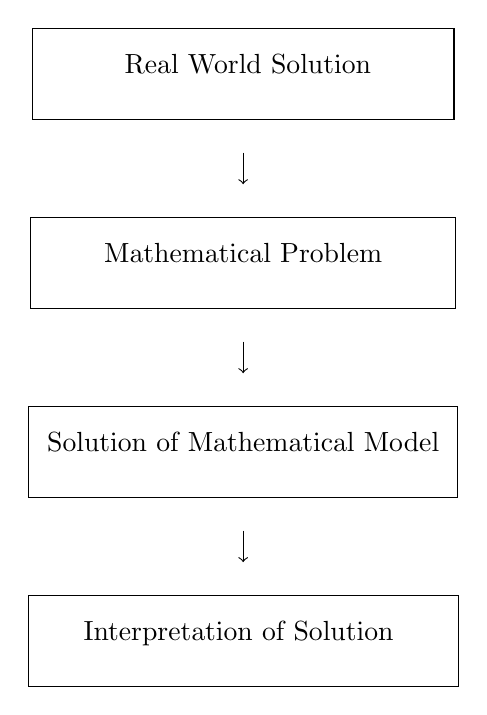
\begin{tikzpicture}
			\node[rectangle, draw, align=center]{\\ ~~~~~~~~~Real World Solution~~~~~~~~~\\};
			\draw[->] (0,-1)--(0,-1.4);
			
			\node[rectangle, draw, align=center] at(0,-2.4){\\ ~~~~~~~Mathematical Problem~~~~~~~~\\};
			\draw[->] (0,-3.4)--(0,-3.8);
			
			\node[rectangle, draw, align=center] at(0,-4.8){\\ ~Solution of Mathematical Model~~\\};
			\draw[->] (0,-5.8)--(0,-6.2);
			
			\node[rectangle, draw, align=center] at(0,-7.2){\\ ~~~~~Interpretation of Solution~~~~~~~\\};
		\end{tikzpicture}
	\end{center}
	
	
	\section{Aim and Objectives of the Study}
	The aim of the project is to solve some ordinary differential equations using finite element method.\sps
	The objectives of this project are to:
	
	\begin{enumerate}
		\item[(i)] examine the solution of ordinary differential equations;
		
		\item[(ii)] show examples of ordinary differential equations using FDM; and
		\item[(iii)] Compare the results with other methods
	\end{enumerate}
	
	
	\section{Outline of the Study}
	This project consists of five chapters. A concise organization of the study is as follows:\sps
	Chapter one contains the general introduction, aim and objectives and definition of relevant terms.\sps
	Chapter two, would focus on solutions to some applications of ODE and examples\sps
	Chapter three would be to show how the summary of the ODEs and the finite difference method could be approximated to the numerical solution of the ODE differential equations.\sps
	Chapter four would use the solution of the ODEs method to find the numerical approximations of Results obtained are compared with the exact solutions where such exists.\sps
	Chapter five presents the summary, conclusion, discussion of the results, and recommendation for further study.
	

	%%%%%%%%%%%%%%%%%%%%%%%%%CHAPTER TWO%%%%%%%%%%%%%%%%%%%%%%%%%%%%
	\chapter{LITERATURE REVIEW}
	\section{Approach to Finite Difference Methods (FDMs)}
	In the literature on numerical analysis, various methods for solving linear and non-linear boundary value problems when solutions cannot be obtained analytically, are available. One of the methods is the iterative method that involves the iterative process. Iterative methods such as the finite difference method (Chawla, 1978), the shooting method (Robert \& Shipman, 1972), the method of exact and truncated (of arbitrary order of accuracy defined by the user) difference schemes (Gavrilyuk \textit{et al.}, 2006) and the integral equation method (Kutniv, 2002) have been developed for obtaining approximate solutions to the boundary value problems. Moreso, a finite difference scheme for second order boundary value problems with a third boundary condition was reported by Kutniv (2002). Equidistant discretization points, and the discretization of the differential equation at an interior point is based on just two evaluations of the function (Pandey, 2010).\sps
	
	\NI One of the approximations of a Taylor series expansion is finite difference method (FDM). A finite difference method is applied on ODE and PDE both. In which each derivative is replaced with an approximate difference formula. The computational domain is usually divided into small sub cells
	and the solution will be obtained at each nodal point. FDM is easy to understand when the physical grid is given in the Cartesian form
	
	
	
	\section{Recent Applications to Numerical Problems Using FDM}
	The problem of the classical boundary layer over a surface has been studied in two different types. First is a boundary layer flow past a stationary surface, while the other type is the problem of a boundary layer flow over a solid surface continuously moving in a fluid at rest such as hot rolling,
	metal forming and continuous casting (Patel \textit{et al.}, 2019).\\
	
	\NI Patel \textit{et al.} (2016) have presented the similarity solution of Magneto hydro dynamic flow of Sisko fluid in semi-infinite flat plate.\\
	
	\NI Mailk \textit{et al.} (2015) and Munir \textit{et al.} (2015) discussed the convective heat transfer of Sisko fluid. The influence of applied magnetic field on Sisko fluid over stretching cylinder was discussed by Mailk \textit{et al.} (2016a). The authors examined the flow characteristics of MHD Sisko fluid over stretching cylinder under the impact of viscous dissipation.\\
	
	\NI Also, Manjunatha and Gireesha (2015), Si \textit{et al.} (2016) and Malik \textit{et al.} (2016b) investigated the fluid flows assuming varying thermal conductivity.\\
	
	\NI Application of FDM on higher order ODE is very rare in the literature. Carlos \textit{et al.} (2011) has presented a numerical solution of the Falkner-Skan equation using high-order and high-ordercompact FDM. Furthermore, Noor \textit{et al.} (2012) introduced FDM in two steps for finding approximate solutions of system of 3rd order boundary value problems associated with odd-order obstacle problems.
	

	%%%%%%%%%%%%%%%%%%%%%%%%%CHAPTER THREE%%%%%%%%%%%%%%%%%%%%%%%%%%%%
	\chapter{METHODOLOGY}
	\section{Introduction}
	In this section, we substituted the derivatives in the ordinary differential equation and in the initial boundary conditions by expressions of approximating derivation formulas. By this approach, we can get an approximating system of equations for the required function values. We illustrated the possibilities of second ODE and Taylor’s series.
	
	
	\section{Description of Finite Difference Method of Second ODE}
	Munir, A., Shahzad, A., \& Khan, M. (2015)\\
	The most general linear second order differential equation is in the form:
	\begin{equation}
		y\dprime(x) + p(x)y\sprime(x) + q(x)y(x) = r(x), ~ a \leq x \leq b \label{eq:3_1}
	\end{equation}
	We need to specify the value of the solution at two distinct points
	\begin{equation*}
		y(a) = A \text{ and } y(b) = B
	\end{equation*}
	These are typically called boundary conditions.\sps
	We can divide the interval $I=[a,b]$ into a chosen number $\mathbf{n}$ of subintervals of equal width.
	\begin{equation*}
		x_i = a + ih~(i=0,1,\ldots, n)
	\end{equation*}
	\begin{center}
		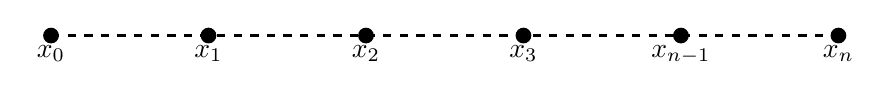
\begin{tikzpicture}
			\draw[thick, dashed] (-2,0)--(8,0);
			\foreach \x / \y in {-2/$x_0$,0/$x_1$,2/$x_2$,4/$x_3$,6/$x_{n-1}$,8/$x_n$}
				\fill (\x,0) circle(0.1) node[below]{\y};
		\end{tikzpicture}
	\end{center}
	Thus, the step size, $h$, of each of the $\mathbf{n}$ is given by
	\begin{equation*}
		h = \frac{b-a}{n}
	\end{equation*}
	We will use the notation to denote $y_i$ the value of the function at the $i$-th node of the computational grid, $y_0 = A$ and $y_n = B$.\sps
	
	\section{Approximation of ODE using FDM}
	First derivative, forward FDM:
	\begin{equation}
		f\sprime(x) = \frac{f(x+h) + f(x)}{h} + O(h) \label{eq:3_2}
	\end{equation}
	First derivative, backward FDM:
	\begin{equation}
		f\sprime(x) = \frac{f(x-h) - f(x)}{h} + O(h) \label{eq:3_3}
	\end{equation}
	First derivative, central FDM:
	\begin{equation}
		f\sprime(x) = \frac{f(x+h) - f(x-h)}{2h} + O(h^2)\label{eq:3_4}
	\end{equation}

	Second derivative, central FD:
	\begin{equation}
		f\dprime(x) = \frac{f(x+h) - 2f(x) + f(x-h)}{h^2} + O(h^2)\label{eq:3_5}
	\end{equation}
	$y_1, y_2,\ldots, y_{n-1}$ can be calculated as follows\sps
	At any mesh point $x=x_i$, the finite-difference representation of the differential equation can be written as follows (based on central FD)
	\begin{eqnarray}
		\frac{y_{i+1} - 2y_i + y_{i-1}}{h^2} + p_i\frac{y_{i+1}-y_{i-1}}{2h}+ q_iy_i = r_i, ~ (i=1,2,\ldots,n-1)\notag \sps
		%%%%%
		2(y_{i+1}-2y_i + y_{i-1})+ hp_i(y_{i+1} - y_{i-1}) + 2h^2q_iy_i = 2h^2r_i,  (i=1,2,\ldots,n-1)~~~~\label{eq:3_6}
	\end{eqnarray}
	
	And arranging the equations with respect to $y_1\ldots,y_n$, we can obtain the system of linear equations.
	\begin{eqnarray}
		(2+hp_i)y_{i+1} + (2h^2q_i - 4)y_i + (2-hp_i)y_{i-1} = 2h^2r_i, (i=1,2,\ldots,n-1)~~~\label{eq:3_7}
	\end{eqnarray}
	The boundary conditions provide of the solution are the two ends of the grid: $y_0=A$ and $y_n=B$.\sps
	We can interpret $y$ as a vector and write the equation formally as an algebraic matrix equation in the form
	\begin{equation}
		A_hY_h = R_h \label{eq:3_8}
	\end{equation}
	\begin{equation*}
		A_k = 
		\begin{bmatrix}
			(2h^2q_1-4) & (2+hp_1) & 0 & \cdots & \cdots & 0\\
			(2-hp_2) & (2h^2q_2 - 4) & (2+hp_3) & 0 & \cdots & 0\\
			0 & (2-hp_3) & (2h^2q_3 - 4) & (2+hp_3) & \cdots & 0 \\
			\vdots & \vdots & \ddots & \ddots & \ddots & \vdots \\
			0 & \cdots & 0 & (2-hp_{n-2}) & (2h^2q_{n-2}) & (2+hp_{n-2})\\
			0 & \cdots & \cdots & 0 & (2-hp_{n-1}) & (2h^2q_{n-1}-4) \\
		\end{bmatrix}
	\end{equation*}
	\begin{equation*}
		R_h = 
		\begin{bmatrix}
			2h^2r_1-(2-hp_1)A\\
			2h^2r_2\\
			2h^2r_3\\
			\vdots\\
			2h^2r_{n-2}\\
			2h^2r_{n-1}-(2+hp_{n-1})B
		\end{bmatrix}
	\end{equation*}
	~\sps
	\begin{equation*}
		Y_h = 
		\begin{bmatrix}
			y_1\\
			y_2\\
			y_3\\
			\vdots\\
			y_{n-2}\\
			y_{n-1}
		\end{bmatrix}
	\end{equation*}
	
	
	\section{Grid Points in Finite Difference Methods Equation}
	In obtaining the finite-difference grid, we subdivided the region into a set of discrete points.\sps
	The spacing between the pints may be uniform or non-uniform.\sps
	
	\NI For example, a grid in the $x$ direction, $x_{\text{min}} \leq x \leq x_{\text{max}}$ may be developed as follows,\sps
	
	\NI We placed a series of $N+1$ nodes numbered from $0$ to $N$ in this region. The coordinate of the first node, $x_0$ equals $x_{\text{min}}$. The final grid node, $x_N = x_{\text{max}}$.\sps
	
	\NI The spacing between any two grid nodes, $x_i$ and $x_{i-1}$, has the symbol $\Delta x_i$. These relations are summarized as equation \refx{3_9}
	\begin{equation}
		\left.
			\begin{array}{c}
				x_0 = x_{\text{min}}\sps
				x_N = x_{\text{max}}\sps
				x_i = x_{i-1}
			\end{array}
		\right\}
		\label{eq:3_9}
	\end{equation}
	A non-uniform grid, with different spacing between different nodes, is illustrated below.
	\begin{center}
		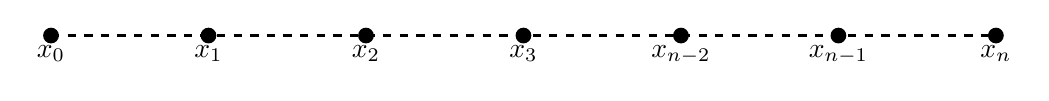
\begin{tikzpicture}
			\draw[thick, dashed] (-4,0)--(8,0);
			\foreach \x / \y in {-4/$x_0$,-2/$x_1$,0/$x_2$,2/$x_3$,4/$x_{n-2}$,6/$x_{n-1}$,8/$x_n$}
				\fill (\x,0) circle(0.1) node[below]{\y};
		\end{tikzpicture}
	\end{center}
	For a uniform grid, all values of $\Delta x_i$ are the same. In this case, the uniform grid spacing, in a one-dimensional problem is usually given the symbol $h$. i.e., $h=x_i = x_{i-1}$ for all the values of $i$.\sps
	
	\NI In two space dimensions, a grid is required for both the $x$ and $y$, directions, which results in the following grid and geometry definitions, assuming that there are $M+1$ grid node in the $y$-direction.
	
	\begin{equation}
		\left.
			\begin{array}{lll}
				x_0 = x_{\text{min}} & x_N = x_{\text{max}} & x_i-x_{i-1}=\Delta x_i\\
				\\
				y_0 = y_{\text{min}} & y_M = y_{\text{max}} & y_j-y_{j-1}=\Delta y_j
			\end{array}
		\right\}
		\label{eq:3_10}
	\end{equation}
	For a three-dimensional transient problem, there would be four independent variables: the three space dimensions, $x, y$ and $z$, and time. Each of these variables would be defined at discrete points. The equation is written in the form of 
	
	\begin{equation}
		\left.
		\begin{array}{lll}
			x_0 = x_{\text{min}} & x_N = x_{\text{max}} & x_i-x_{i-1}=\Delta x_i\\
			y_0 = y_{\text{min}} & y_M = y_{\text{max}} & y_j-y_{j-1}=\Delta y_j\\
			\\
			z_0 = z_{\text{min}} & z_k = z_{\text{max}} & z_k-z_{k-1}=\Delta z_k\\
			t_0 = t_{\text{min}} & t_n = t_{\text{max}} & t_n-t_{n-1}=\Delta t_n
		\end{array}
		\right\}
		\label{eq:3_11}
	\end{equation}
	Any dependent variable such as $u(x,y,z,t)$ in a continuous representation would be defined only at discrete grid points in a finite-difference representation. The following notation is used for the set of discrete values of dependent variables.
	\begin{equation*}
		u_{ijk}^n = u(x_i,y_j,z_k,t_n)
	\end{equation*}
	For steady-state problems, the $n$ superscript is omitted. For problems with only one or two space dimensions, two or one of the directional subscripts may be omitted. The general us of the notation remains. The subscripts (and superscript) on the dependent variable represent a particular point in the region, $(x_i,y_j,z_k,t_n)$ where the variable is defined. 
	
	\section{Taylor's Series Expression of Finite Difference Method}
	Pandey, P. K. (2010)\\
	In this case, we obtained the approximation of FDM using Taylor's series.\sps
	
	\NI Since Taylor series for a function of one variable, therefore $f(x)$, expanded about some point $x=a$, is given by the infinite series,
	\begin{equation}
		f(x) = f(a) + \frac{df}{dx}\Big|_{x=a} (x-a) + \frac{1}{2!}\frac{d^2f}{dx^2}\Big|_{x=a} (x-a)^2 +  \frac{1}{3!}\frac{d^3f}{dx^3}\Big|_{x=a} (x-a)^3 + \cdots \label{eq:3_12}
	\end{equation}
	The $x=a$ subscript on the derivatives reinforces the fact that these derivatives are evaluated at the expansion point, $x=a$.\sps
	
	\NI We the write the summation notation as follows:
	\begin{equation}
		f(x) = \sum_{n=0}^{\infty}\frac{1}{n!}\frac{d^nf}{dx^n}\Big|_{x=a}(x-a)^n \label{eq:3_13}
	\end{equation}
	In the equation \refx{3_13}, we use the definitions of $0!=1!=!$ and the definition of the zeroth derivative as the function itself. i.e.,
	\begin{equation*}
		\frac{d^0f}{dx^0}\Big|_{x=a} = f(a)
	\end{equation*}
	If the series is truncated after some finite number of terms, say $m$ terms, the omitted terms are called the remainder in mathematical analysis and the truncation error in numerical analysis.\sps
	
	\NI These omitted terms are also an infinite series. This is expressed in equation \refx{3_14}
	\begin{eqnarray}
		f(x) = \sum_{n=0}^{m}\frac{1}{n!}\frac{d^nf}{dx^n}\Big|_{x=a}(x-a)^n  &+& \sum_{n=m+1}^{\infty}\frac{1}{n!}\frac{d^nf}{dx^n}\Big|_{x=a}(x-a)^n \label{eq:3_14}\sps
		\text{Terms used}~~~~~~~~ & + & ~~~~\text{Truncation error}\notag
	\end{eqnarray}
	in this equation, the second sum presents the truncation error, $\epsilon_m$, from truncating the series after $m$ terms.
	\begin{equation}
		\epsilon_m = \sum_{n=m+1}^{\infty}\frac{1}{n!}\frac{d^nf}{dx^n}\Big|_{x=a}(x-a)^n\label{eq:3_15}
	\end{equation}
	The theorem of the mean can be used to show that the infinite-series truncation error can be expressed in terms of the first term in the truncation error, that is 
	\begin{equation}
		\epsilon_m =\frac{1}{(m+1)!}\frac{d^{m+1}f}{dx^{m+1}}\Big|_{x=\xi}(x-a)^{m+1}\label{eq:3_16}
	\end{equation}
	
	%%%%%%%%%%%%%%%%%%%%%%%%%CHAPTER FOUR%%%%%%%%%%%%%%%%%%%%%%%%%%%%
	\chapter{DEMONSTRATION OF ORDINARY DIFFERENTIAL EQUATIONS EXAMPLES USING FINITE DIFFERENCE METHOD}
	
	\section{Introduction}
	In this section, some numerical examples of Ordinary Differential Equation were solved using the Finite Difference Method as the basis function
	
	
	\section{Demonstration of ODEs using FDM}
	\subsection*{Example 4.1}
	A quadrilateral element (left) and the dimensionless representation of the quadrilateral as a square in terms of the dimensionless variables $\xi$ and $\eta$.
	\begin{center}
		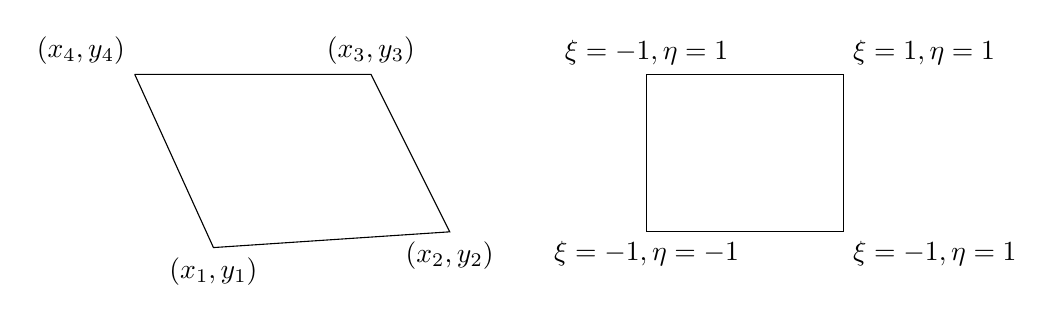
\begin{tikzpicture}		
			\draw (0,2)node[above left]{($x_4,y_4$)}--(3,2)node[above]{$(x_3,y_3)$}--(4,0)node[below]{$(x_2,y_2)$}--(1,-0.2)node[below]{$(x_1,y_1)$}--(0,2);
			
			\draw (6.5,2)node[above]{$\xi=-1, \eta=1$}--(9,2)node[above right]{$\xi=1, \eta=1$}--(9,0)node[below right]{$\xi=-1, \eta=1$}--(6.5,0)node[below]{$\xi=-1, \eta=-1$}--(6.5,2);
		\end{tikzpicture}
	\end{center}
	In the Figure above, the quadrilateral represents an individual element in a two-dimensional finite element scheme.\\
	
	\NI This general quadrilateral can be mapped into a square element shown on the right of the figure. In this region the dimensionless coordinates, $\xi$ and $\eta$, range from –1 to +1. (The lower limit is chosen to be –1 rather than zero to facilitate a numerical integration technique known
	as Gauss integration.)\\
	
	\NI The actual coordinates, $x$ and $y$, are related to the dimensionless coordinates as follows.
	\begin{eqnarray}
		x = \frac{x_1(1-\xi)(1-\eta) + x_2(1-\xi)(1+\eta) + x_3(1+\xi)(1+\eta) + x_4(1-\xi)(1+\eta)}{4}~~\label{eq:4_1}\spn{0.6}
		%%%%%%%
		y = \frac{y_1(1-\xi)(1-\eta) + y_2(1-\xi)(1+\eta) + y_3(1+\xi)(1+\eta) + y_4(1-\xi)(1+\eta)}{4}~~\label{eq:4_2}
	\end{eqnarray}
	\newpage
	\begin{eqnarray}
		\frac{dy}{dx}\Big|_{x=x_0} = \frac{y(x_0+h) - y(x_0 -h)}{2h}  = \frac{a+b(x_0+h) + c(x_0+h)^2 - [a+b(x_0-h) + c(x_0 - h)^2]}{2h} \notag\spn{0.6}
		= \frac{2bh + c(x_0^2 + 2x_0h + h^2)-c(x_0^2-2x_0h + h^2)}{2h}=\frac{2bh + 4cx_0h}{2h} = b+2cx_0~~~~~~~~~~~~~\notag
	\end{eqnarray}
	In equations \refx{4_1} and \refx{4_2}, setting $\xi$ and $\eta$ to the values of any corner of the coordinate system will give the correct value for the x and y coordinates of the corner. These x and y coordinates are known from the starting process of the finite element analysis where a grid is generated for a particular geometry.\sps
	
	\NI The variable, $\varphi$, which satisfies a differential equation to be solved numerically, is approximated by some polynomial over the element. A different polynomial is used for each element. The simplest polynomial to use in the two-dimensional case is the same polynomial that is used for the coordinate system. This type of an element, where the same polynomial approximations are used for both the coordinates and the unknown function is called an isoparametric element.
	\begin{equation}
		\varphi = \frac{\varphi_1(1-\xi)(1-\eta) + \varphi_2(1-\xi)(1+\eta) + \varphi_3(1+\xi)(1+\eta) + \varphi_4(1-\xi)(1+\eta)}{4}\label{eq:4_3}
	\end{equation}
	
	\subsection*{Example 4.2}
	Consider the one-dimensional problem shown in Equation \refx{4_4}
	\begin{equation}
		\frac{d^2T}{dx^2}+a^2T = 0 ~~ \text{with}~~ T=T_A ~~\text{at}~~ x=0 ~~\text{and}~~ T=T_B ~~\text{at}~~ x = L\label{eq:4_4}
	\end{equation}
	To solve this problem using a finite-difference approach, we replace the differential equation by a finite-difference analog. We will use a uniform, one-dimensional grid in the $x$ direction.\\
	
	\NI Using $N+1$ nodes on the grid, $(0-N)$,\\
	
	\NI The step size, $h$,
	\begin{equation}
		\frac{L-0}{N}\label{eq:4_5}
	\end{equation}
	The second derivative in FDM.
	\begin{equation}
		\frac{T_{i+1} + T_{i-1} - 2T_i}{h^2} + a^2 T_i = 0\label{eq:4_6}
	\end{equation}
	Using boundary conditions
	\begin{equation*}
		T_0=T_A ~~~\text{and}~~~~ T_N = T_B
	\end{equation*}
	\begin{eqnarray}
		(a^2h^2)T_1 + T_2 &=& - T_A \notag \sps
		T_1 + (a^2h^2)T_2 + T_3 &=& 0\notag\sps
		T_2 + (a^2h^2)T_3 + T &=& 0\notag
	\end{eqnarray}
	$(N-8)$ additional similar equation with $T_4$ through $T_{N-4}$ multiplied by $(a^2h^2)$ go here.
	\begin{align*}
		(N-4)T_{N-4} + (a^2h^2)T_{N-3} + T_{N-2} &= 0 \\
		(N-3)T_{N-3} + (a^2h^2)T_{N-2} + T_{N-1} & = 0 \\
		(N-2)T_{N-2} + (a^2h^2)T_{N-1} &= -T_B
	\end{align*}
	We see that we have to solve $N-2$ simultaneous linear algebraic equations for the unknown temperatures $T_1$ to $T_{N-1}$.\\
	
	\NI The set of equations that we have to solve is a simple one since each equation is a relationship among only three temperatures.\\
	
	\NI None of the other temperatures on the grid are unknowns here. We cannot solve the equation until we specify numerical values for the boundary temperatures, $T_A$ and $T_B$, and the length, $L$.\\
	
	\NI We also need to specify a value for $N$.\\
	
	\NI This will give the value of $\dsp h = \frac{(L – 0)}{N}$.\\
	
	\NI Before specifying $a, T_A, T_B, L$, and $N$, we want to examine the exact solution of Equation \refx{4_4}, which is given by Equation \refx{4_7}.\\
	
	\NI You can substitute this equation into Equation \refx{4_4} to show that the differential equation is satisfied. You can also set $x = 0$ and $x = L$ in Equation \refx{4_7} to show that this solution satisfies and the boundary conditions.
	\begin{equation}
		T = \frac{T_B - T_A\cos(aL)}{\sin(aL)}\sin(ax) + T_A\cos(ax)\label{eq:4_7}
	\end{equation}
	We can obtain the exact solution of equation \refx{4_7} without specifying values for $a, T_A, T_B$, and $L$. However, we have to specify these values (as well as a value of $x$) to compute a numerical value for $T$. In the numerical solution process, we cannot obtain an analytical form like equation \refx{3_5}; instead, we must specify numerical values for the various parameters before we start to solve the set of algebraic equations shown above.\\
	
	\NI For this example, we choose $a = 2, T_A = 0, T_B = 1$, and $L = 1$; we can then determine the solution for different values of $N$. Table \ref{tb:4_1} compares the exact and numerical solution for $N = 10$.\\
	
	\NI The error in Table \ref{tb:4_1} is defined as the absolute value of the difference between the exact and the numerical solution. This error is seen to vary over the solution domain. At the boundaries, where the temperatures are known, the error is zero. As we get further from the boundaries, the error increases, becoming a maximum at the midpoint of the region.\sps
	\begin{longtable}{ccccc}
		\caption{Comparison of Exact and Numerical Solution for Equation \refx{4_4}}\\
		\label{tb:4_1}\spn{-1} \hline
		$i$ & $x$ & Exact Solution & Numerical Solution & Error\\
		0 & 0 & 0 & 0 & 0\\
		1 & 0.1 & 0.21849 & 0.21918 & 0.00070\\
		2 & 0.2 & 0.42826 & 0.42960 & 0.00134\\
		3 & 0.3 & 0.62097 & 0.62284 & 0.00187\\
		4 & 0.4 & 0.78891 & 0.79115 & 0.00224\\
		5 & 0.5 & 0.92541 & 0.92783 & 0.00242\\
		6 & 0.6 & 1.02501 & 1.02739 & 0.00238\\
		7 & 0.7 & 1.08375 & 1.08585 & 0.00211\\
		8 & 0.8 & 1.09928 & 1.10088 & 0.00160\\
		9 & 0.9 & 1.07099 & 1.07188 & 0.00089\\
		10 & 1 & 1 & 1 & 0\\ \hline
	\end{longtable}
	
	\NI In problems with a large number of numerical results, it is useful to have a single measure of the error. (This is a typical problem any time we desire a single measure for a set of numbers. In the parlance of vectors, we speak of the vector norm as a single number that characterizes the size of the vector. We can use a similar terminology here and speak of the norm of the error.) Two measures of the overall error are typically used. The first is the largest absolute error.\\
	
	\NI For the data in Table \ref{tb:4_1}, that error is $0.00242$. Another possible definition of the error norm is the root-mean-square (RMS) error, defined as in Equation \refx{4_8}. In that equation, $N$ refers to the number of values that contribute to the error measure; boundary temperatures, which are given, not calculated, would not be included in the sums.
	\begin{equation}
		\Big|\epsilon\Big|_{RMS} = \sqrt{\frac{1}{N}\sum_{i=1}^{N}\epsilon_i^2} = \sqrt{\frac{1}{N}\sum_{i=1}^{N}(T_{exact}-T_{numerical})_i^2} \label{eq:4_8}
	\end{equation}
	The data in Table \ref{tb:4_1} have nine unknown temperatures.\\
	
	\NI Plugging the data for those temperatures into equation \refx{4_11} and using $N = 9$, gives the RMS error as 0.00183. If we repeat the solution using $N = 100$, the maximum error is 0.0000241, and the RMS error is 0.0000173. In both measures of the error we have achieved a reduction
	in error by a factor of 100 as we decrease the grid spacing by a factor of 10. This is an indication of the second-order error that we used in converting the differential equation into a finite difference equation.\\
	
	\NI An important problem in computational fluid dynamics and heat transfer is determining the gradients at the wall that provide important physical quantities such as the heat flux. We want to examine the error in the heat flux in the problem that we have solved.\\
	
	\NI We first have to calculate the exact solution for the heat flux. Since this problem involved heat generation, we will also be interested in the integrated (total) heat generation over the region. The wall gradients of the exact solution in equation in Equation \refx{4_4} can be found by taking
	the first derivative of that solution.
	\begin{equation}
		\frac{dT}{dx}=a\frac{T_B-T_A\cos(aL)}{\sin(aL)}\cos(ax) - aT_A\sin(ax)\label{eq:4_9}
	\end{equation}
	The boundary heat transfer at $x = 0$ and $x = L$ is found by evaluating this expression at those points and multiplying by the thermal conductivity, $k$.
	\begin{equation}
		q_{x=L} = -k\frac{dT}{dx}\Big|_{x=L} = -ka\frac{T_B - T_A\cos(aL)}{\sin(aL)}\cos(aL) + kaT_A\sin(aL) \label{eq:4_10}
	\end{equation}
	
	\begin{eqnarray}
		q_{x=0} &=& -k\frac{dT}{dx}\Big|_{x=0} = -ka\frac{T_B - T_A\cos(aL)}{\sin(aL)}\cos(0) + kaT_A\sin(0)\notag \sps
		&=& -ka\frac{T_B - T_A\cos(aL)}{\sin(aL)} \label{eq:4_11}
	\end{eqnarray}
	Equation \refx{4_10} can be simplified by using a common denominator, $\sin(aL)$, and using the trig identity that $\sin^2x + \cos^2x = 1$.
	\begin{equation}
		q_{x=L} = \frac{ka}{\sin(aL)}\Big[T_A\cos^2(aL) - T_B\cos(aL) + T_A\sin^2(aL)\Big] = \frac{ka\big[T_A - T_B\cos(aL)\big]}{\sin(aL)}\label{eq:4_12}
	\end{equation}
	The heat flow at $x = 0$ is entering the region; the heat flow at $x = L$ is leaving the region. The total heat leaving the region, $qx = L-qx = 0$ must be equal to the total heat generated. Since the heat source term for the differential equation was equal to $bT$, the total heat generation for the region, Qgen tot, must be equal to the integral of $bT$ over the region. Using the exact solution in equation \refx{4_4} we find the total heat generated as follows.
	\begin{equation}
		Q_{gen tot} = \int_0^L bTdx = b\int_0^L\Biggl[\frac{T_B - T_A\cos(aL)}{\sin(aL)}\sin(ax) + T_A\cos(ax)\Biggr]dx \label{eq:4_13}
	\end{equation}
	
	\NI Performing the indicated integration and evaluating the result at the specified upper and lower limits gives the following result.
	\begin{equation}
		Q_{gen tot} = \frac{b}{a}\Biggl[\frac{T_B - T_A\cos(aL)}{\sin(aL)}\Big(1-\cos(aL)\Big)+ T_A\sin(aL)\Biggr]\label{eq:4_14}
	\end{equation}
	We can simplify this slightly by using a common denominator of $\sin(aL)$ and using the same trig identity, $\sin^2x + \cos^2x = 1$, used previously.
	
	\subsection*{Example 4.3}
	Consider the second-order ODE equation of the form
	\begin{equation}
		\frac{d^2y}{dx^2} = f(x,y,y\sprime), ~~ a \leq x \leq b \label{eq:4_15}
	\end{equation}
	with the Boundary conditions
	\begin{equation*}
		y(a) = y_a ~~~~\text{ and } ~~~~ y(b) = y_b
	\end{equation*}
	Equation \refx{4_15} may be regarded as initial value problem. Assuming a simply supported load.
	\begin{equation}
		\frac{d^2y}{dx^2} = \frac{qx(L-x)}{2EI}\label{eq:4_16}
	\end{equation}
	Another for of simply supported beam,
	\begin{equation}
		\frac{d^2y}{dx^2} - \frac{Ty}{EI} = \frac{qx(L-x)}{2EI} \label{eq:4_17}
	\end{equation}
	$x$ = location along the beam (in)\\
	$T$ = tension applied (lbs)\\
	$E$ = Young’s modulus of elasticity of the beam (psi)\\
	$I$ = second moment of area (in4 )\\
	$q$ = uniform loading intensity (lb/in)\\
	$L$ = length of beam (in)
	
	\begin{center}
		\includegraphics[width=1\textwidth]{beam.png}
	\end{center}
	Imposed conditions
	\begin{eqnarray}
		y(x=0) &=& 0\notag\sps
		y(x=L) &=& 0\notag
	\end{eqnarray}
	Here, we solved equation \refx{4_17} given $T = 7200, Q =5400, L= 75, E = 30$, and $I =120$\sps
	Substituting the given values,
	\begin{equation*}
		\frac{d^2y}{dx^2} - \frac{7200y}{(3 \times 10^6)(120)}=\frac{(500)\times(75-x)}{2(3\times 10^6)120}
	\end{equation*}
	\begin{equation*}
		\frac{d^2y}{dx^2}-2 \times 10^{-6}y = 7.5 \times 10^{-7}x(75-x)
	\end{equation*}
	Approximating the derivative $\dsp\frac{d^2y}{dx^2}$ at node $i$ by the central divided difference approximation
	\begin{center}
		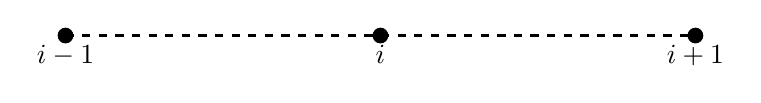
\begin{tikzpicture}
			\draw[thick, dashed] (0,0)--(8,0);
			\foreach \x / \y in {0/$i-1$,4/$i$,8/$i+1$}
				\fill (\x,0) circle(0.1)node[below]{\y};
		\end{tikzpicture}
	\end{center}
	\begin{equation*}
		\frac{d^2y}{dx^2} \approx \frac{y_{i+1} - 2y_i + y_{i-1}}{(\Delta x)^2}
	\end{equation*}
	We can rewrite the equation as
	\begin{equation*}
		\frac{y_{i+1} - 2y_i + y_{i-1}}{(\Delta x)^2} - 2 \times 10^{-6}y_i = 7.5 \times 10^{-7}x_i(75-x_i)
	\end{equation*}
	
	Since $\Delta x = 25$, we can now represent it as 4 nodes
	\begin{center}
		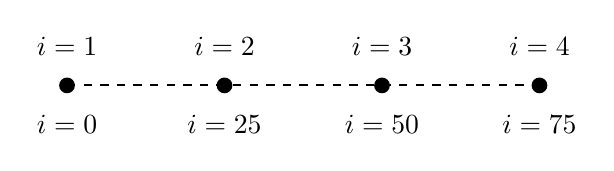
\begin{tikzpicture}
			\draw[thick,dashed] (0,0)--(6,0);
			\foreach \x in {0,2,4,6}
				\fill (\x,0) circle(0.1);
			
			\foreach \x / \y in {0/1,2/2,4/3,6/4}
				\node at(\x,0.5){$i=\y$};
			
			\foreach \x / \y in {0/0,2/25,4/50,6/75}
				\node at(\x,-0.5){$i=\y$};
		\end{tikzpicture}
	\end{center}
	The location of the 4 nodes is then
	\begin{eqnarray}
		x & = & 0\notag\sps
		x_1 & = & x_0 + \Delta x = 0 + 25 = 25\notag\sps
		x_2 & = & x_1 + \Delta x = 25 + 25 = 50\notag\sps
		x_3 & = & x_2 + \Delta x = 50 + 25 = 75\notag
	\end{eqnarray}
	We then rewrite the equation at each node, we get\sps
	\ubt{Node 1}: For a simply supported beam at boundary condition
	\begin{equation*}
		x = 0, y = 0
	\end{equation*}
	\ubt{Node 2}
	\begin{eqnarray}
		\frac{y_3 - 2y_2 + y_1}{(25)^2} -2 \times 10^{-6}y_2 = 7.5 \times 10^{-7}x_2(75-x_2)\notag\sps
		0.0016y_1 - 0.003202y_2 + 0.0016y_3 = 9.375 \times 10^{-4}\notag
	\end{eqnarray}
	\ubt{Node 3}
	\begin{eqnarray}
		\frac{y_4 - 2y_3 + y_2}{(25)^2} -2 \times 10^{-6}y_3 = 7.5 \times 10^{-7}x_3(75-x_3)\notag\sps
		0.0016y_2 - 0.003202y_3 + 0.0016y_4 = 9.375 \times 10^{-4}\notag
	\end{eqnarray}
	\ubt{Node 4}
	\begin{equation*}
	\text{At}~~~x = 75, ~~ y_4 = 0
	\end{equation*}
	The Nodes 1-4 can now be solved simultaneously since we have 4 unknowns.\\
	This is written in matrix form
	\begin{equation*}
		\begin{bmatrix}
			1 & 0 & 0 & 0\\
			0.0016 & -0.003202 & 0.0016 & 0\\
			0 & 0.0016 & -0.003202 & 0.0016\\
			0 & 0 & 0 & 1
		\end{bmatrix}
		\begin{bmatrix}
			y_1\\
			y_2\\
			y_3\\
			y_4
		\end{bmatrix}
		=
		\begin{bmatrix}
			0\\
			9.375 \times 10^{-4}\\
			9.375 \times 10^{-4}\\
			0
		\end{bmatrix}
	\end{equation*}
	From the tridiagonal matrix, we can apply iterative method e.g. Guass-Siedel method,
	\begin{equation*}
		\begin{bmatrix}
			y_1\\
			y_2\\
			y_3\\
			y_4
		\end{bmatrix}
		=
		\begin{bmatrix}
			0\\
			-0.5852\\
			-0.5852\\
			0\\
		\end{bmatrix}
	\end{equation*}
	~\\
	\begin{equation*}
		y(50) = y(x_2) \approx y_2 = -0.5852
	\end{equation*}
	The exact solution of the ordinary differential equation is derived as follows. The homogeneous part of the solution is given by solving the characteristic equation
	\begin{eqnarray}
		m^2 - 2 \times 10^{-6} = 0\notag\sps
		m = \pm 0.0014142\notag
	\end{eqnarray}
	So, we can write the equation in the form of
	\begin{equation*}
		y_h = K_1 e^{0.0014142x} + K_2e^{-0.0014142x}
	\end{equation*}
	Particular part of the solution
	\begin{equation}
		y_p = A_x^2 + B_x + C \label{eq:4_18}
	\end{equation}
	We substituted Equation \refx{4_18} into \refx{4_17}, we obtained
	\begin{equation*}
		\frac{d^2y_p}{dx^2}(Ax^2 + Bx + C)- 2\times 10^{-6}(Ax^2 + Bx + C) = 7.5 \times 10^{-7}x(75-x)
	\end{equation*}
	\begin{eqnarray}
		A &=& 0.375\notag\sps
		B &=& -28.125\notag\sps
		C &=& 3.75 \times 10^5\notag
	\end{eqnarray}
	Particular solution is then written as
	\begin{equation}
		y_p = 0.375x^2 - 28.125x + 3.75 \times 10^5 \label{eq:4_19}
	\end{equation}
	Complete solution is then given by
	\begin{equation}
		y = 0.375x^2 - 28.125x + 3.75 \times 10^5 + K_1 e^{0.0014142x} + K_2 e^{-0.0014142x} \label{eq:4_20}
	\end{equation}
	Applying the following boundary conditions
	\begin{eqnarray}
		y(x=0) =0\notag\sps
		y(x=75) = 0\notag
	\end{eqnarray}
	The system of equations becomes
	\begin{align*}
		K_1 + K_2 &= -3.75 \times 10^5\sps
		1.1119K_1 + 0.89937K_2 &=-3.75 \times 10^5
	\end{align*}
	These equations are represented in matrix form by
	\begin{equation*}
		\begin{bmatrix}
			1.1119 & 1 \\
			0.89937 & 1 
		\end{bmatrix}
		\begin{bmatrix}
			K_1\\
			K_2
		\end{bmatrix}
		=
		\begin{bmatrix}
			-3.75 \times 10^5\\
			-3.75 \times 10^5
		\end{bmatrix}
	\end{equation*}
	We solved the unknown variables using Gaussian elimination method
	\begin{equation*}
		\begin{bmatrix}
			K_1\\
			K_2
		\end{bmatrix}
		=
		\begin{bmatrix}
			-1.775656226 \times 10^5\\
			-1.974343774 \times 10^5
		\end{bmatrix}
	\end{equation*}
	We substituted these values back into equation \refx{4_20}
	\begin{eqnarray}
		y &=& 0.375x^2 - 28.125x + 3.75 \times 10^5 - 1.775656226\times 10^5e^{0.0014142x}\notag\\
		&-& 1.97434774 \times 10^5 e^{-0.0014142x}\notag
	\end{eqnarray}
	The above expression for the deflection of the beam is displayed with a larger number of significant digits. This is done to minimize the round-off error because the above expression involves subtraction of large numbers that are close to each other.\\
	
	\NI The relative true error is calculated. In doing this, we calculated the exact solution for the
	equation at $y = 50$
	\begin{eqnarray}
		y(50) &=& 0.375(50)^2 - 28.125(50) + 3.75 \times 10^5 - 1.775656226 \times 10^5 e^{0.0014142(50)} \notag\\
		&-&1.974343774 \times 10^5 e^{-0.0014142(50)}\notag \\
		y(50) &=& -0.5320\notag
	\end{eqnarray}
	Therefore, the true error is estimated by
	\begin{eqnarray}
		E_t &=& \text{Exact Value} - \text{Approximate Value}\notag\sps
		E_t &=& -0.5320 - (-0.5852)\notag\sps
		E_t &=& 0.05320\notag
	\end{eqnarray}
	The relative true error is given by
	\begin{eqnarray}
		\epsilon_i &=& \frac{\text{True Error}}{\text{True Value}} \times 100\%\notag\sps
		\epsilon_i &=& \frac{0.05320}{-0.5320} \times 100\%\notag\sps
		\epsilon_i &=& -10\%\notag
	\end{eqnarray}
	
	
	\subsection*{Example 4.4}
	Consider the thermal equation
	\begin{equation}
		\frac{d^2T}{dx^2}+a^2T=0 ~~~\text{with}~~ T=T_A ~~\text{at}~~ x=0 ~~\text{and}~~ T=T_B ~~\text{at}~~ x = L\label{eq:4_21}
	\end{equation}
	We solved the equation using Galerkin’s method (weighted residual) of finite difference.\\
	
	\NI In applying finite elements to a one-dimensional problem.
	\begin{equation}
		\int_0^L w_i(x)\Biggl[\frac{d^2\hat{T}}{dx^2}+a^2\hat{T}\Biggr]dx = 0 ~~~~~ 1=1,\ldots,N \label{eq:4_22}
	\end{equation}
	Consider the region of the equation $x=0$ and $x=L \leq N$\sps
	We used a simple linear polynomial approximation for the temperature.\sps
	$\hat{T}$, is approximation symbol;\sps
	$T$ is the true temperature,\sps
	
	\NI Substituting our polynomial approximation into the differential equation, we can write a differential equation based on the approximation functions.
	\begin{equation}
		\hat{T} = \sum_{i=1}^{N}T_i\phi_i(x) \label{eq:4_23}
	\end{equation}
	The general property of the equation is given as
	\begin{equation}
		\varphi_i(xj) = \delta_{ij}\label{eq:4_24}
	\end{equation}
	$i^{th}$ shape function is one at the point $x=x_i$ and is zero at all other nodal points $x_j$, where $j \neq i$.\sps
	
	\NI Given $\hat{T}_i = T_i$ at the nodal points. The shape functions can have values other than zero and one at other $x$ values that do not occur at nodes.\sps
	The shape function is given for this equation is
	\begin{equation}
		\varphi_i(x) = 
		\left\{
			\begin{array}{ll}
				0 & x \leq x_{i-1}\sps
				\dsp \frac{x-x_{i-1}}{x_i - x_{i-1}} & x_{i-1} \leq x \leq x_i\sps
				\dsp \frac{x_{i+1}-x}{x_{i+1} - x_i} & x_i \leq x \leq x_{i+1}\sps
				0 & x \geq x_{i+1}
			\end{array}
		\right. \label{eq:4_25}
	\end{equation}
	Generally shape function is related as non-zero only for the two elements that border the node with the coordinate $x_i$.\sps
	
	\NI Therefore, we plotted the figure below relative to the shape function.\sps
	\begin{center}
		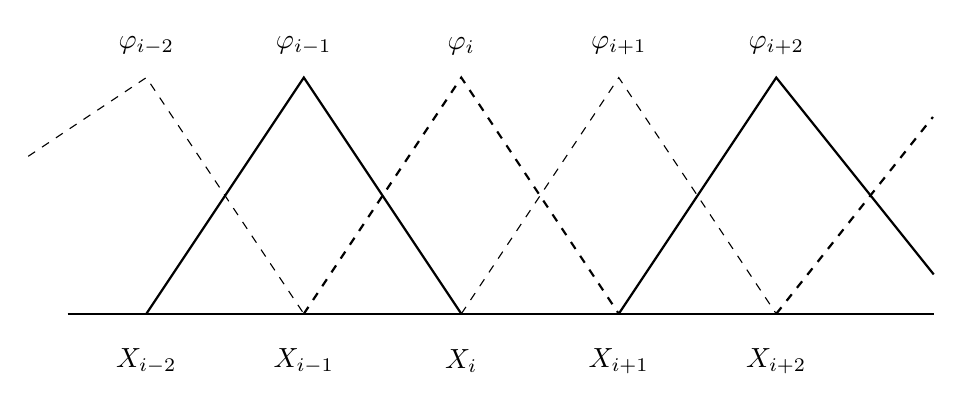
\begin{tikzpicture}
			\draw[thick] (-1,0)--(10,0);
			
			\draw[dashed] (-1.5,2)--(0,3)--(2,0);
			
			\draw[dashed, thick] (2,0)--(4,3)--(6,0);
			
			\draw[thick] (6,0)--(8,3)--(10,0.5);
			
			%%%second
			\draw[thick](0,0)--(2,3)--(4,0);
			\draw[dashed] (4,0)--(6,3)--(8,0);
			\draw[dashed, thick] (8,0)--(9.99,2.5);
			
			%%nodes
			\foreach \x / \y in {0/i-2,2/{i-1}, 6/{i+1}, 8/{i+2}}
			{
				\node at (\x,3.4){$\varphi_{\y}$};
				\node at (\x,-0.6){$X_{\y}$};	
			}
			\node at (4,3.4){$\varphi_{i}$};
			\node at (4,-0.6){$X_{i}$};
		\end{tikzpicture}
	\end{center}
	\begin{eqnarray}
		\phi_i &=& 0 (x=x_{i-1})\notag\sps
		x &=& x_i \notag\sps
		x &=& x_{i-1} \notag\sps
		\phi_i(x_j) &=& \delta_{ij}\notag
	\end{eqnarray}
	Over a single element, say the one between $x_i$ and $x_{i+1}$, there are only two shape functions that are nonzero: $\phi_i$ and $\phi_{i+1}$.\\
	
	\NI We applied the Garlekin’s analysis to obtain a set of algebraic equations for unknown values of temperature $T$.\sps
	
	\NI Tridiagonal matrix equations of unknown values is $T_i$\sps
	
	\NI Differentiating and integrating Equations \refx{4_26} and \refx{4_27}
	\begin{equation*}
		\hat{T} = T_1\varphi_I(x) + T_{II}\varphi_{II}(x) = T_I \frac{x_{II}-x}{x_{II} - x_I} + T_{II}\frac{x-x_{I}}{x_{II} - x_I} ~~~~~ x_I \leq x \leq x_{II}
	\end{equation*}
	$I$ and $II$, for the two ends of our element
	For the Galerkin method we re-write Equation \refx{4_22} as
	\begin{equation}
		\int_{x_I}^{x_{II}}\varphi_i\Biggl[\frac{d^2\hat{T}}{dx^2}+ a^2\hat{T}\Biggr]dx = 0 ~~~~~ i=I, II \label{eq:4_26}
	\end{equation}
	Applying integration by parts to Equation \refx{4_26} to get rid of the second derivative, the general form of integration by parts takes the form of Equation \refx{4_27}
	\begin{equation}
		\int_a^budv = uv\Biggl|_a^a - \int_a^bvdu \label{eq:4_27}
	\end{equation}
	We have to manipulate the second derivative term in equation \refx{4_26} to get it into the form shown in \refx{4_27}. We do this by noting that the second derivative is just the derivative of the first derivative and we can algebraically cancel dx terms as shown below.
	\begin{equation}
		\int_{x_{I}}^{x_{II}} \varphi_i\frac{d^2\hat{T}}{dx^2}dx = \int_{x_{I}}^{x_{II}}\varphi_i \frac{d}{dx}\frac{d\hat{T}}{dx} dx = \int_{x_{I}}^{x_{II}}\varphi_i d\Biggl[\frac{d\hat{T}}{dx}\Biggr]\label{eq:4_28}
	\end{equation}
	The final integral in equation \refx{4_28} has the form of the integration by parts formula in equation \refx{4_27} We can identify $u=\varphi_i$, and $v=\dsp \frac{d\hat{T}}{dx}$. Using these definitions of u and v in equation \refx{4_27} gives the following result.
	
	\begin{equation}
		\int_{x_{I}}^{x_{II}}\varphi_i\frac{d^2\hat{T}}{dx^2} dx = \varphi_i\frac{d\hat{T}}{dx}\Biggl|_{x_{I}}^{x_{II}} - \int_{x_{I}}^{x_{II}}\frac{d\varphi_i}{dx}d\hat{T} = \varphi_i\frac{d\hat{T}}{dx}\Biggl|_{x_{I}}^{x_{II}} - \int_{x_{I}}^{x_{II}}\frac{d\varphi_i}{dx}\frac{d\hat{T}}{dx}dx \label{eq:4_29}
	\end{equation}
	With this result, we can rewrite equation \refx{4_26} as follows.
	\begin{equation}
		\varphi_i\frac{d\hat{T}}{dx}\Biggl|_{x_{I}}^{x_{II}} -\int_{x_{I}}^{x_{II}}\frac{d\varphi_i}{dx}\frac{d\hat{T}}{dx}dx + \int_{x_{I}}^{x_{II}} a^2 \varphi_i\hat{T} dx = 0 ~~~~ i=I, II \label{eq:4_30}
	\end{equation}
	We need to evaluate this equation using the linear shape functions in equation \refx{4_25} that we have selected for this analysis. The shape functions have the following first derivatives for the element under consideration. Once the derivatives of the shape functions are known we can compute the derivatives of the approximate temperature. In taking the derivatives of the approximate temperature polynomial, we consider the nodal values, $T_I$ and $T_{II}$, to be constants.
	\begin{equation}
		\frac{d\varphi_I}{dx}= \frac{-1}{x_{II}-x_I}~~~~~\text{and}~~~~~ \frac{d\varphi_{II}}{dx} = \frac{1}{x_{II}-x_I}\label{eq:4_31}
	\end{equation}
	\begin{equation*}
		\frac{d\hat{T}}{dx} = T_I\frac{d\hat{T}_I}{dx} + T_{II}\frac{d\hat{T}_{II}}{dx} = \frac{-T_{I}}{x_{II} - x_I}+\frac{T_{II}}{x_{II} - x_I} = \frac{T_{II}- T_I}{x_{II} - x_I}
	\end{equation*}
	We can substitute the temperature polynomial and the shape functions, and their derivatives, into equation \refx{4_30} We will show the details for $\varphi = \varphi_i$, on a term-by-term basis, starting with the first term in equation \refx{4_30}.\sps
	
	\NI The shape function, $\varphi_I$, is zero at the upper limit of this evaluation, $x = x_{II}$ so we only have the lower limit where $\varphi_I = 1$. Rather than substituting the interpolation polynomial for the approximate temperature gradient, we replace this term by the actual gradient. We can then handle boundary conditions that use this gradient. If we do not have a gradient boundary condition, we can use the resulting equations to compute the gradient.
	\begin{equation}
		\varphi\frac{d\hat{T}}{dx}\Biggl|_{x_{I}}^{x_{II}} = \frac{x_{II} - x}{x_{II} - x_I}\frac{d\hat{T}}{dx}\Biggl|_{x_{I}}^{x_{II}} = \frac{x_{II} - x}{x_{II} - x_I}\frac{dT}{dx}\Biggl|_{x=II}-\frac{x_{II} - x}{x_{II} - x_I}\frac{dT}{dx}\Biggl|_{x=I} = - \frac{dT}{dx}\Biggl|_{x=I} \label{eq:4_32}
	\end{equation}
	The middle integral with two derivative terms becomes the simple integral of a constant
	\begin{equation}
		\int_{x_{I}}^{x_{II}}\frac{d\varphi_I}{dx}\frac{d\hat{T}}{dx}dx = \int_{x_{I}}^{x_{II}}\frac{-1}{x_{II} - x_I}\frac{T_{II} - T_I}{x_{II} - x_I}dx = - \frac{T_{II} - T_I}{(x_{II}-x_I)^2}x\Biggl|_{x_I}^{x_{II}} = -\frac{T_{II} - T_I}{x_{II} - x_I} \label{eq:4_33}
	\end{equation}
	The final term in equation \refx{4_30} requires the most work for integration. The last step in this integration is left as an exercise for the interested reader.
	\begin{equation}
		\begin{array}{l}
			\dsp\int_{x_{I}}^{x_{II}}a^2\varphi_I\hat{T} dx = a^2\int_{x_{I}}^{x_{II}}\frac{x_{II}- x}{x_{II} - x_I}\Biggl[T_I\frac{x_{II} - x}{x_{II} - x_I} + T_{II}\frac{x-x_I}{x_{II} - x_I}\Biggr] dx\spn{0.5}
			%%%
			\dsp = \frac{a^2}{(x_{II}-x_I)^2}\int_{x_{I}}^{x_{II}}\Biggl[T_I(x_{II}-x)^2 + T_{II}(x-x_I)(x_{II}-x)\Biggr]dx\spn{0.5}
			%%%%
			\dsp= \frac{a^2}{6}(2T_I + T_{II})(x_{II} - x_I)
		\end{array}
		\label{eq:4_34}
	\end{equation}
	We can substitute the results of equations \refx{4_32} to \refx{4_34} back into equation \refx{4_30} to get the result for using the left shape function, $\varphi_I$, as the weighting function.
	\begin{equation}
		\begin{array}{l}
			\dsp \varphi_I\frac{d\hat{T}}{dx}\Biggl|_{x_I}^{x_{II}} - \int_{x_{I}}^{x_{II}}\frac{d\varphi_{I}}{dx}\frac{d\hat{T}}{dx}dx + \int_{x_{I}}^{x_{II}}a^2\varphi_{I}\hat{T} dx - \frac{dT}{dx}\Biggl|_{x=x_I}\spn{0.8}
			%%%%%%%
			\dsp+ \frac{T_{II} - T_I}{x_{II} - x_I} + \frac{a^2}{6}(2T_I + T_{II})(x_{II}-x_I) = 0 
		\end{array}\label{eq:4_35}
	\end{equation}
	If we rearrange the last equation in \refx{4_35} (4.34) we get the following relationship between $T_I$ and $T_{II}$ (and the gradient at $x = x_I$) for our element, based on using $\varphi_{I}$ as the weighting function.
	\begin{equation}
		T_I\Biggl(\frac{a^2}{3}(x_{II}-x_I)-\frac{1}{x_{II} - x_I}\Biggr) + T_{II}\Biggl(\frac{a^2}{6}(x_{II}-x_I)+\frac{1}{x_{II} - x_I}\Biggr) = \frac{dT}{dx}\biggl|_{x=x_I}\label{eq:4_36}
	\end{equation}
	If we repeat the analysis that led to equation \refx{4_35} , using $\varphi_{II}$ as the weighting function, we get the following result, in place of equation \refx{4_35}
	\begin{equation}
		\begin{array}{l}
			\dsp \varphi_{II}\frac{d\hat{T}}{dx}\Biggl|_{x_I}^{x_{II}} - \int_{x_{I}}^{x_{II}}\frac{d\varphi_{II}}{dx}\frac{d\hat{T}}{dx}dx + \int_{x_{I}}^{x_{II}}a^2\varphi_{II}\hat{T} dx - \frac{dT}{dx}\Biggl|_{x=x_II}\spn{0.8}
			%%%%%%%
			\dsp- \frac{T_{II} - T_I}{x_{II} - x_I} + \frac{a^2}{6}(T_I + 2T_{II})(x_{II}-x_I) = 0 
		\end{array}\label{eq:4_37}
	\end{equation}
	Rearranging this equation gives us the second relationship between $T_I$ and $T_{II}$ for our elements; this one contains the gradient at $x = x_{II}$.
	\begin{equation}
		T_I\Biggl(\frac{a^2}{6}(x_{II}-x_I)+\frac{1}{x_{II} - x_I}\Biggr) + T_{II}\Biggl(\frac{a^2}{3}(x_{II}-x_I)-\frac{1}{x_{II} - x_I}\Biggr) =- \frac{dT}{dx}\biggl|_{x=x_{II}}\label{eq:4_38}
	\end{equation}
	There are only two different coefficients in equations \refx{4_36} and \refx{4_38}. We can simplify the writing of these equations by assigning a separate symbol for the two different coefficients.
	\begin{equation}
		\alpha = \Biggl(\frac{a^2}{3}(x_{II}-x_I)-\frac{1}{x_{II} - x_I}\Biggr)~~~~~ \beta = \Biggl(\frac{a^2}{6}(x_{II}-x_I)+\frac{1}{x_{II} - x_I}\Biggr) \label{eq:4_39}
	\end{equation}
	With these definitions, we can write our element equations, \refx{4_36} and \refx{4_38} as follows.
	\begin{equation}
		\alpha T_I + \beta T_{II} = \frac{dT}{dx}\Biggl|_{x=x_I} ~~~~~~~\beta T_I + \alpha T_{II} =- \frac{dT}{dx}\Biggl|_{x=x_{II}} \label{eq:4_40}
	\end{equation}
	We have this pair of equations for each of our elements. We need to consider how the element equations all fit together to construct a system of equations for the region. To do this we return to the global numbering system for the region that was used in the finite-difference analysis.\\
	
	\NI In the global system, the first element lies on the left-hand boundary, between $x_0$ and $x_1$. The next element lies between $x_1$ and $x_2$. We start by writing the element equations in \refx{4_40} for these two elements using the global numbering scheme. For the first element, the element
	index, $I$, corresponds to the global index 0 and the element index $II$ corresponds to the global index 1. With this notation, the element equations in \refx{4_40} become.
	\begin{equation}
		\alpha_0 T_0 + \beta_0 T_{1} = \frac{dT}{dx}\Biggl|_{x=x_0} ~~~~~~~\beta_0 T_0 + \alpha_0 T_{1} =- \frac{dT}{dx}\Biggl|_{x=x_{1}} \label{eq:4_41}
	\end{equation}
	Here we have added a subscript to the coefficients $\alpha$ and $\beta$. In the global scheme, the element sizes may be different. To account for this we have to use a global index for the $\alpha$ and $\beta$ coefficients as shown below.
	\begin{equation}
		\alpha_i = \Biggl(\frac{a^2}{3}(x_{i+1}-x_i)-\frac{1}{x_{i+1} - x_i}\Biggr)~~~~~ \beta_i = \Biggl(\frac{a^2}{6}(x_{i+1}-x_i)+\frac{1}{x_{i+1} - x_i}\Biggr) \label{eq:4_42}
	\end{equation}
	Both equations in \refx{4_41} have the boundary temperature, $T_0$, and the first equation has the temperature gradient on the left-hand boundary. In this example, we know that the boundary temperature is given as $T_0 = T_A$ from the boundary condition from the original problem in equation \refx{4_4}. However the boundary gradient (at $x = x_0$) is unknown in our example. In problems with other kinds of boundary conditions we may know the boundary gradient, but not $T_0$ or we may have a second relationship between $T_0$ and the boundary gradient.\\
	
	\NI The second equation in \refx{4_41} has an internal gradient as one of the terms. We can eliminate this gradient term by examining the element equations for the second element, written in the global numbering system. From equation \refx{4_40}, we have the following equations for the second element.
	\begin{equation}
		\alpha_1 T_1 + \beta_1 T_{2} = \frac{dT}{dx}\Biggl|_{x=x_1} ~~~~~~~\beta_1 T_1 + \alpha_1 T_{2} =- \frac{dT}{dx}\Biggl|_{x=x_{2}} \label{eq:4_43}
	\end{equation}
	We eliminate the temperature gradient at $x = x_1$ by adding the second equation from the equation pair in \refx{4_43} to the first equation in \refx{4_45}. This gives the following equation.
	\begin{equation}
		\beta_0T_0 + (\alpha_0 + \alpha_1)T_1 + \beta_1T_2 = 0 \label{eq:4_44}
	\end{equation}
	\newpage
	\section{Table of Results}
	\begin{longtable}{lcccc}
		\caption{Computation of errors using FDM to Solution in Equation \refx{4_25}}\\
		\label{tb:4_2}\spn{-1}\hline
		Heating Parameter & \multicolumn{2}{c}{$a=2$} & \multicolumn{2}{c}{$a=0.2$}\\ \hline 
		Grid Elements & $N=100$ & $N=10$ & $N=100$ & $N=10$\\
		Method & FDM & FDM & FDM & FDM\\
		RMS Error in T & 1.73E-05	&1.83E-03 & 6.21E-10 & 6.52E-08\\
		Maximum error in T & 2.41E-05 & 2.42E-03 & 8.62E-10 & 8.60E-08\\[0.4cm]
		Error in $\dsp \frac{dT}{dx}\Big|_{x=0}$ & 3.63E-04 & 3.62E-02 & 1.34E-06 & 2.25E-07\\[0.4cm]
		Error in $\dsp \frac{dT}{dx}\Big|_{x=L}$ & 2.14E-04 & 1.79E-02 & 1.31E-06 & 4.46E-07 \\[0.4cm] \hline
	\end{longtable}
	
	
	
	
	
	
	
	
	
	
	
	
	
	
	
	
	
	
	
	
	
	%%%%%%%%%%%%%%%%%%%%%%%%%CHAPTER FIVE%%%%%%%%%%%%%%%%%%%%%%%%%%%%
	\chapter{SUMMARY, CONCLUSION AND RECOMMENDATION}
	
	\section{Summary and Conclusion}
	In this project work, Finite Difference Method provides two different approaches to the numerical analysis of differential equations. In a broad sense, each of these approaches are a method for converting a differential equation, that applies to every point in a region, to a set of algebraic equations that apply at a set of discrete points in the domain.
	
	
	\section{Discussion of the Results}
	The coefficients in the algebraic equations, using a finite difference method, are based on the use of finite difference expressions that apply at individual points on a grid. For examples 4.1 to 4.4, it is considered a one-dimensional problem and the algebraic equations were particularly simple to solve. In multidimensional problems, we will have a more complex set of differential equations to solve. The error of the heating parameter is presented in tabular form.\\
	
	\NI We observed that Finite difference expressions can be derived from Taylor series. This approach leads to an expression for the truncation error that provides us with knowledge of how this error depends on the step size. This is called the order of the error.\\
	
	\NI Finite Difference Method is a tradeoff between higher order and required work. In principle, there should be different combinations of order and grid spacing that gives the same accuracy. A higher order finite-difference expression should require fewer grid nodes to get the same
	accuracy
	

	\section{Recommendation}
	From the obtained results, I recommend the use of Finite Difference Method for Ordinary Differential Equations using differential equations as basic functions and this can be extended to solve other equations such as finite element and partial differential equations. The basic question is how much extra work is required to use the higher order expressions compared to
	repeating the work for the lower order expressions more frequently on a finer grid.\\
	
	\NI In finite-difference approaches, we need to be concerned about both truncation errors and roundoff errors. Therefore, modern computers with higher bits could be utilized for routine calculations as in the case of ODEs using FDM.
	
	
	\chapter*{REFERENCES}
	\addcontentsline{toc}{chapter}{REFERENCES}
	\begin{description}
		\item Carlos, D. D.,~- Duncan, L. \& Carlos, G. (2011). Numerical solution of the Falkner-Skan equation using third-order and high-order-compact finite difference schemes. \tti{J. of the Braz. Soc. of Mech. Sci. \& Eng.}, 33(4), 381-392.
		
		
		\item Chawla, M. M. (1978). A fourth order tridiagonal finite difference method for general twopoint boundary value problems with mixed boundary conditions. \textit{J. Inst. Maths. Applics.},
		21 (1978): 83.
		
		
		\item Gavrilyuk, I. P., ~Herman, M., ~Kutniv, M. V. \& Makarov, V. L. (2006). Difference schemes for non-linear boundary value problems using Runge — Kutta IVP-solvers. \textit{Advances in Difference Equation}, 12167(2006): 1–29.
		
		
		\item Kutniv, M. V. (2002). Three-point difference schemes of high accuracy order for second order ordinary differential equations with boundary conditions of third kind. \textit{Visnyk of the Lviv Univ., Series Applied Mathematics and Computer Science}, (2002)4: 61–66.
		
		
		\item Malik, M. Y., ~Arif, H., ~Salahuddin T. \& Awais, M. (2016a). Effects of viscous dissipation on MHD boundary layer flow of Sisko fluid over a stretching cylinder. \textit{AIP Advances} 6(035009).
		
		
		\item Malik, M. Y., ~Arif, H., ~Salahuddin T., ~Awais, M., ~\& Bilal, S. (2016b). Magneto hydro dynamic flow of Sisko fluid over a stretching cylinder with variable thermal conductivity: A numerical study. \textit{AIP Advances} 6(025316).
		
		
		\item Manjunatha, S., ~and Gireesha, B. J. (2015). Effects of variable viscosity and thermal conductivity on MHD flow and heat transfer of a dusty fluid. \textit{Ain Shams Engineering Journal.}, 7(1): 505-515
		
		
		\item Munir, A., ~Shahzad, A., ~\& Khan, M. (2015). Convective Flow of Sisko Fluid over a Bidirectional Stretching Surface. PLOS ONE, 10(6), 1-13. doi:10.1371/journal.pone.0130342
		
		
		\item Noor, M. A., ~Al-Said, E., ~\& Noor, K. I. (2012). Finite difference method for solving a system of third-order boundary value problems. \textit{Journal of Applied Mathematics, 2012, 1–10}. doi:10.1155/2012/351764
		
		
		\item Pandey, P. K. (2010). Finite difference method for a second-order ordinary differential equation with a boundary condition of the third kind. \textit{Journal of Computational Methods in Applied Mathematics}, 10(1): 109-116.
		
		
		\item Patel M., ~Patel, J., ~\& Timol, M. G. (2019). Numerical solution of 3rd order ode using fdm: on a moving surface in MHD flow of Sisko fluid. \textit{Applications and Applied Mathematics: An International Journal (AAM)}, 14(1), 284-295.
		
		
		\item Patel, J., ~Patel, M., \& Timol, M.G. (2016). Magneto hydro dynamic flow of Sisko fluid. \textit{ARS - Journal of Applied Research and Social Sciences}. 3(14): 45-55.
		
		
		\item Roberts, S. M., ~Shipman, J. S. (1972). Two-point boundary value problems, Shooting Methods. \textit{Elsevier}, 1972.
		
		
		\item Si, X., ~Zhu, X., ~Zheng, L., ~Zhang, X., and Lin P. (2016). Laminar film condensation of pseudoplastic non-Newtonian fluid with variable thermal conductivity on an isothermal vertical plate. \textit{International Journal of Heat and Mass Transfer}, 92: 979–986.
		
		
	\end{description}
\end{document}

